% Created 2020-03-12 Thu 20:27
% Intended LaTeX compiler: pdflatex
\documentclass[10pt, compress, aspectratio=169, xcolor={table,usenames,dvipsnames}]{beamer}

\usepackage{booktabs}
\mode<beamer>{\usetheme[numbering=fraction, progressbar=none, titleformat=smallcaps, sectionpage=none]{metropolis}}
\usepackage{sourcecodepro}
\usepackage{booktabs}
\usepackage{array}
\usepackage{listings}
\usepackage{graphicx}
\usepackage[english]{babel}
\usepackage[scale=2]{ccicons}
\usepackage{url}
\usepackage{relsize}
\usepackage{amsmath}
\usepackage{bm}
\usepackage{wasysym}
\usepackage{ragged2e}
\usepackage{textcomp}
\usepackage{pgfplots}
\usepackage{multirow}
\usepgfplotslibrary{dateplot}
\definecolor{Base}{HTML}{191F26}
\definecolor{Highlight}{HTML}{ffda99}
\definecolor{Accent}{HTML}{bb0300}
\setbeamercolor{alerted text}{fg=Accent}
\setbeamercolor{frametitle}{bg=Base}
\setbeamercolor{normal text}{bg=black!2,fg=Base}
\setsansfont[BoldFont={Source Sans Pro Semibold},Numbers={OldStyle}]{Source Sans Pro}
\lstdefinelanguage{Julia}%
{morekeywords={abstract,struct,break,case,catch,const,continue,do,else,elseif,%
end,export,false,for,function,immutable,mutable,using,import,importall,if,in,%
macro,module,quote,return,switch,true,try,catch,type,typealias,%
while,<:,+,-,::,/},%
sensitive=true,%
alsoother={$},%
morecomment=[l]\#,%
morecomment=[n]{\#=}{=\#},%
morestring=[s]{"}{"},%
morestring=[m]{'}{'},%
}[keywords,comments,strings]%
\lstset{ %
backgroundcolor={},
basicstyle=\ttfamily\scriptsize,
breakatwhitespace=true,
breaklines=true,
captionpos=n,
commentstyle=\color{Accent},
extendedchars=true,
frame=n,
keywordstyle=\color{Accent},
language=R,
rulecolor=\color{black},
showspaces=false,
showstringspaces=false,
showtabs=false,
stepnumber=2,
stringstyle=\color{gray},
tabsize=2,
}
\renewcommand*{\UrlFont}{\ttfamily\smaller\relax}
\graphicspath{{../../img/}}
\addtobeamertemplate{block begin}{}{\justifying}
\usetheme{default}
\author{\footnotesize Pedro Bruel \newline \scriptsize \emph{phrb@ime.usp.br}}
\date{\scriptsize \today}
\title{Introduction to Linear Regression}
\hypersetup{
 pdfauthor={\footnotesize Pedro Bruel \newline \scriptsize \emph{phrb@ime.usp.br}},
 pdftitle={Introduction to Linear Regression},
 pdfkeywords={},
 pdfsubject={},
 pdfcreator={Emacs 26.3 (Org mode 9.2.5)},
 pdflang={English}}
\begin{document}

\maketitle

\section{Introduction}
\label{sec:orgfa2e2a7}
\begin{frame}[label={sec:org3bdbb34}]{Describing Experimental Data in Computer Science}
\begin{columns}
\begin{column}{0.5\columnwidth}
\begin{block}{A Performance Optimization Problem}
\begin{itemize}
\item A \alert{program} with \alert{parameters} \(X \in \mathcal{X}\)
\item A \alert{performance metric} \(f: \mathcal{X} \mapsto \mathbb{R}\)
\item What is the \(X_*\) that \alert{minimizes} \(f(\cdot)\)?
\end{itemize}

\begin{block}{Dealing with Experimental Data}
\begin{itemize}
\item We can't measure \(f(\cdot)\) \alert{precisely}:
\begin{itemize}
\item Interference from network, other programs, OS, random fluctuations, \dots{}
\end{itemize}
\item Fortunately, we can \alert{model} \(f(\cdot)\):
\begin{itemize}
\item \alert{Linear models}
\item Neural networks
\item \dots{}
\end{itemize}
\end{itemize}
\end{block}
\end{block}
\end{column}

\begin{column}{0.5\columnwidth}
\begin{center}
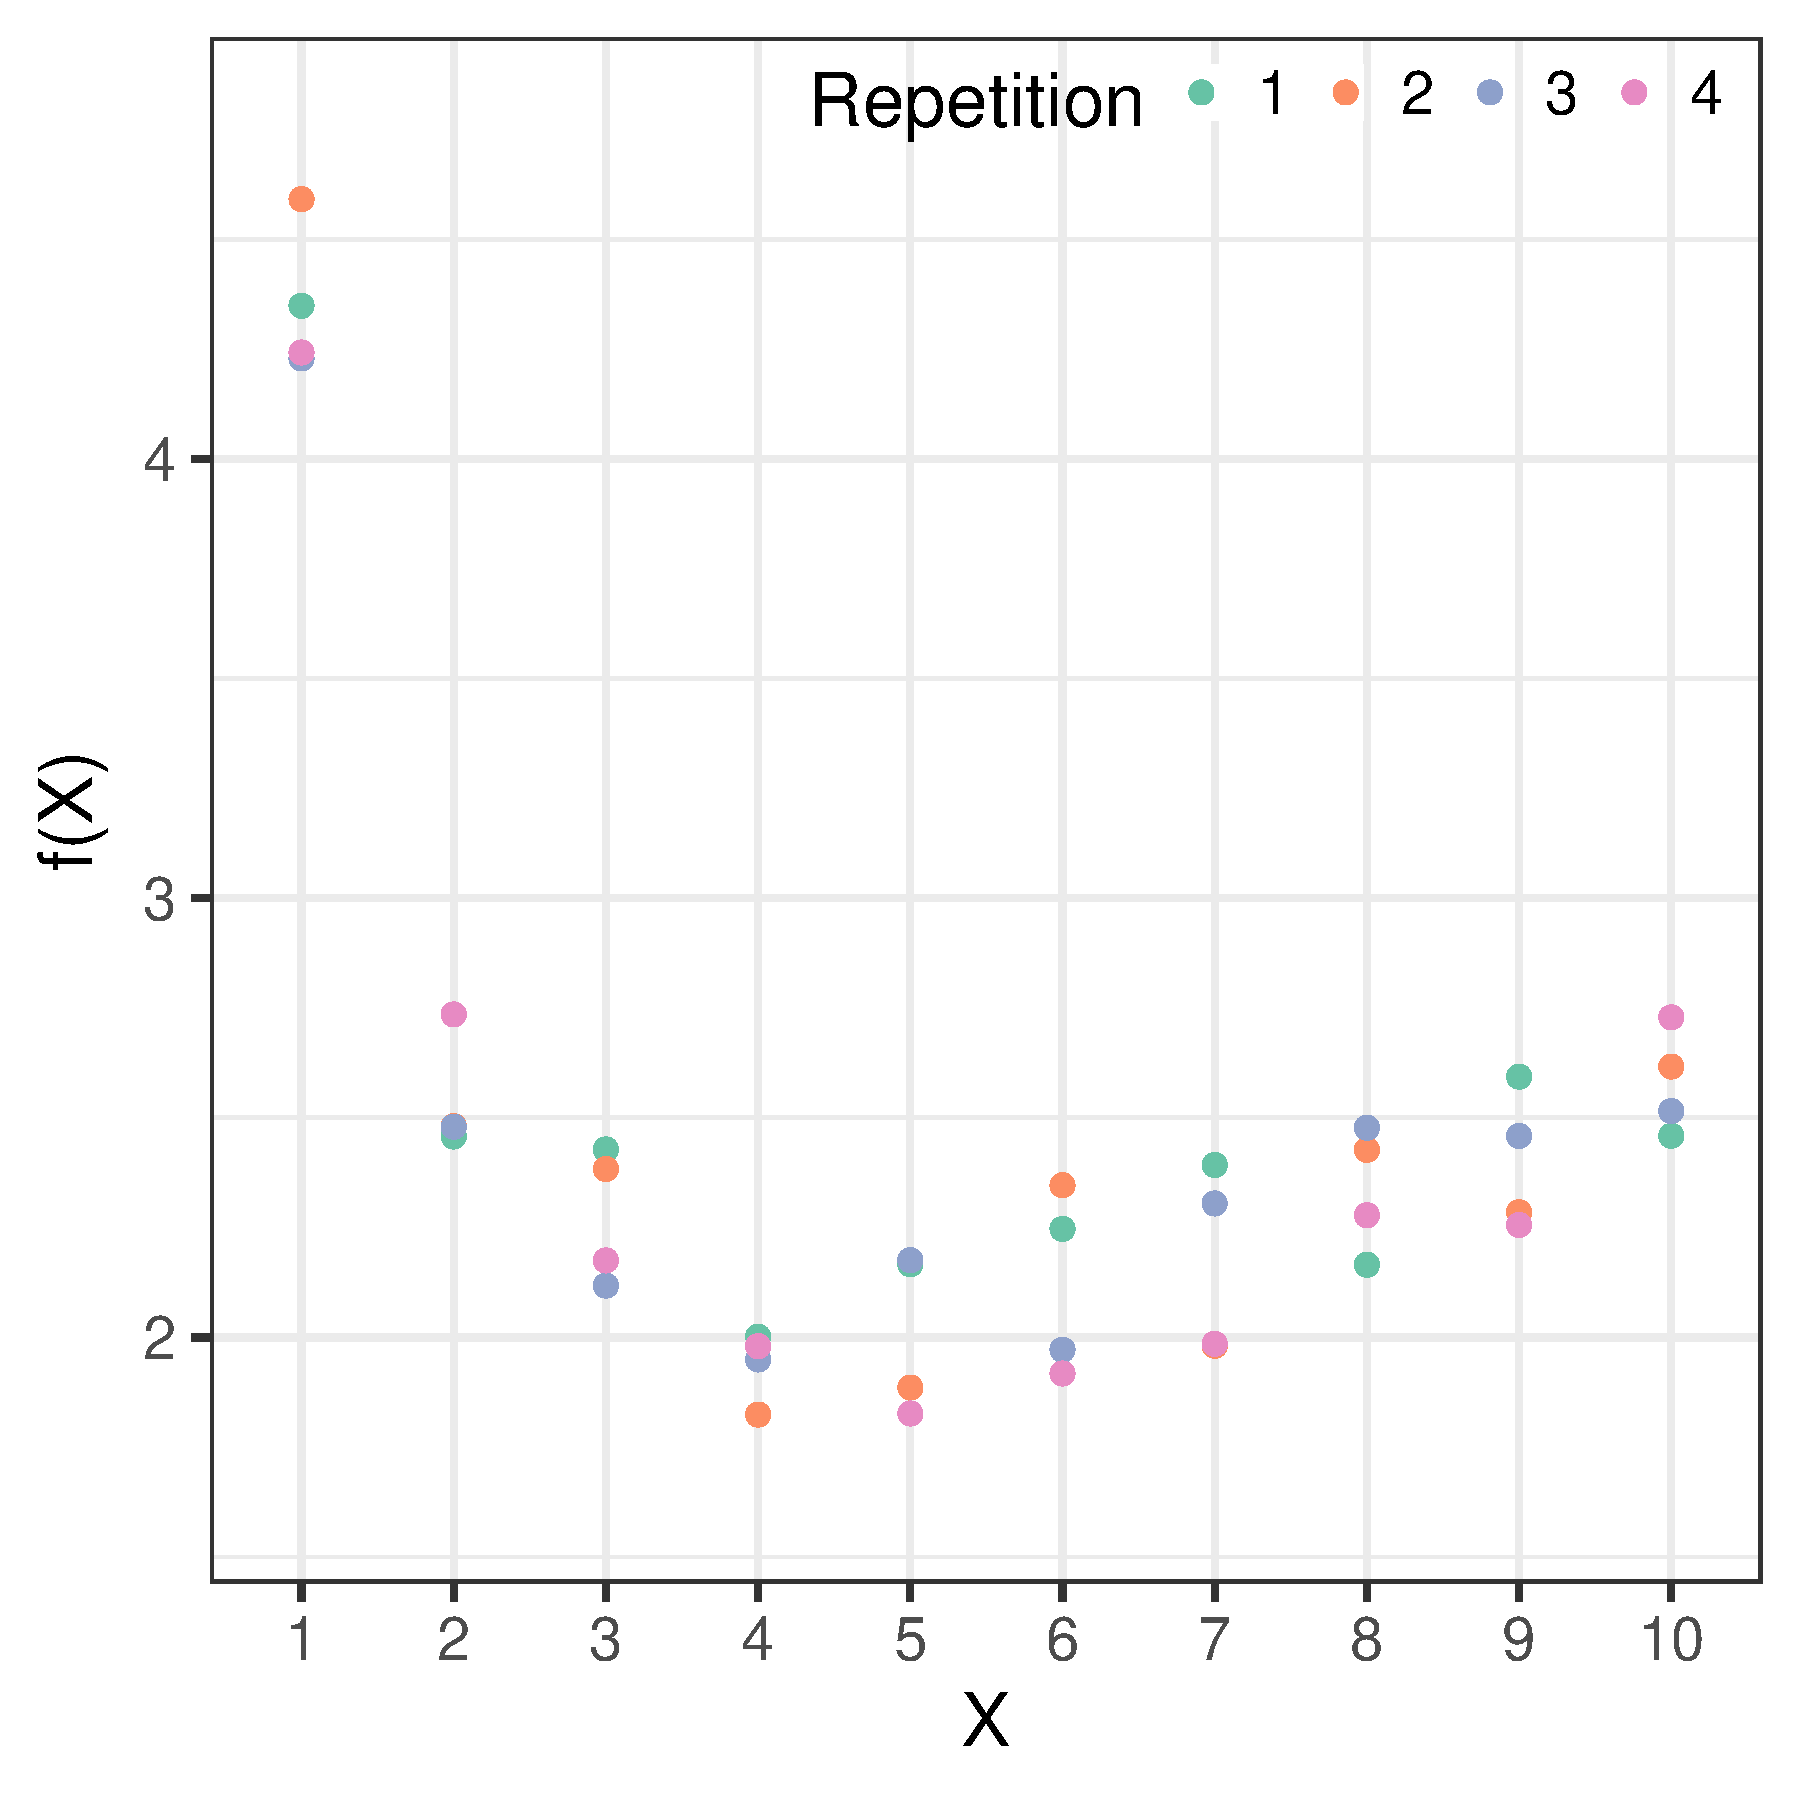
\includegraphics[width=\columnwidth]{../../../img/intro-linear-regression-experimental-data.pdf}
\end{center}
\end{column}
\end{columns}
\end{frame}

\begin{frame}[label={sec:org7ba86d2}]{Describing Experimental Data in Computer Science}
\begin{columns}
\begin{column}{0.5\columnwidth}
\begin{block}{A Statistical Linear Model for \(f(X)\)}
\vspace{0.2em}
\[
    \mathbf{Y} = \mathcal{M}(\mathbf{X})\theta(\mathbf{X}) + \boldsymbol{\varepsilon}
    \]

\only<1>{
Where, for \alert{\(n\) experiments} and \alert{\(k\) parameters}:
\begin{itemize}
\item \(\mathbf{X} \in \mathcal{X}\): explanatory variables
\item \(\mathbf{Y} \in \mathbb{R}^{n\times{}1}\): response, or explained variable
\item \(\mathcal{M}: \mathcal{X} \mapsto \mathbb{R}^{n\times{}k}\): model matrix
\item \(\theta: \mathcal{X} \mapsto \mathbb{R}^{k\times{}1}\): model parameters
\item \(\boldsymbol{\varepsilon} \in \mathbb{R}^{n\times{}1}\): model error
\end{itemize}
}
\only<2>{
Where, for \alert{\(40\) experiments} and \alert{\(1\) parameter}:
\begin{itemize}
\item \(\mathbf{X} \in \mathcal{X}\): \(\{\mathbf{x}_j, \; \mathbf{x}_j = (1,\dots,10)\}_{j = 1,\dots,4}\)
\item \(\mathbf{Y} \in \mathbb{R}^{40\times{}1}\): \(\{y_i, \; y_i = f(\mathbf{X}_i)\}_{i = 1,\dots,40}\)
\item \(\mathcal{M}: \mathcal{X} \mapsto \mathbb{R}^{40\times{}1}\): \(\mathbf{1}^{40\times{}1}\)
\item \(\theta: \mathcal{X} \mapsto \mathbb{R}^{1\times{}1}\): \(\theta_0\)
\item \(\boldsymbol{\varepsilon} \in \mathbb{R}^{40\times{}1}\): \(\mathbf{Y} - \mathcal{M}(\mathbf{X})\theta(\mathbf{X})\)
\end{itemize}
}
\only<3>{
Where, for \alert{\(40\) experiments} and \alert{\(2\) parameters}:
\begin{itemize}
\item \(\mathbf{X} \in \mathcal{X}\): \(\{\mathbf{x}_j, \; \mathbf{x}_j = (1,\dots,10)\}_{j = 1,\dots,4}\)
\item \(\mathbf{Y} \in \mathbb{R}^{40\times{}1}\): \(\{y_i, \; y_i = f(\mathbf{X}_i)\}_{i = 1,\dots,40}\)
\item \(\mathcal{M}: \mathcal{X} \mapsto \mathbb{R}^{40\times{}2}\): \(\left[ \mathbf{1}^{40\times{}1} \; | \; \mathbf{X} \right]\)
\item \(\theta: \mathcal{X} \mapsto \mathbb{R}^{2\times{}1}\): \([\theta_{0}, \theta_{1}]\)
\item \(\boldsymbol{\varepsilon} \in \mathbb{R}^{40\times{}1}\): \(\mathbf{Y} - \mathcal{M}(\mathbf{X})\theta(\mathbf{X})\)
\end{itemize}
}
\only<4>{
Where, for \alert{\(40\) experiments} and \alert{\(3\) parameters}:
\begin{itemize}
\item \(\mathbf{X} \in \mathcal{X}\): \(\{\mathbf{x}_j, \; \mathbf{x}_j = (1,\dots,10)\}_{j = 1,\dots,4}\)
\item \(\mathbf{Y} \in \mathbb{R}^{40\times{}1}\): \(\{y_i, \; y_i = f(\mathbf{X}_i)\}_{i = 1,\dots,40}\)
\item \(\mathcal{M}: \mathcal{X} \mapsto \mathbb{R}^{40\times{}2}\): \(\left[ \mathbf{1}^{40\times{}1} \; | \; \mathbf{X} \; | \; \{x^{2}, \; x \in \mathbf{X}\} \right]\)
\item \(\theta: \mathcal{X} \mapsto \mathbb{R}^{2\times{}1}\): \([\theta_{0}, \theta_{1}, \theta_{2}]\)
\item \(\boldsymbol{\varepsilon} \in \mathbb{R}^{40\times{}1}\): \(\mathbf{Y} - \mathcal{M}(\mathbf{X})\theta(\mathbf{X})\)
\end{itemize}
}
\only<5>{
Where, for \alert{\(40\) experiments} and \alert{\(3\) parameters}:
\begin{itemize}
\item \(\mathbf{X} \in \mathcal{X}\): \(\{\mathbf{x}_j, \; \mathbf{x}_j = (1,\dots,10)\}_{j = 1,\dots,4}\)
\item \(\mathbf{Y} \in \mathbb{R}^{40\times{}1}\): \(\{y_i, \; y_i = f(\mathbf{X}_i)\}_{i = 1,\dots,40}\)
\item \(\mathcal{M}: \mathcal{X} \mapsto \mathbb{R}^{40\times{}2}\): \(\left[ \mathbf{1}^{40\times{}1} \; | \; \mathbf{X} \; | \; \{\frac{1}{x}^{}, \; x \in \mathbf{X}\} \right]\)
\item \(\theta: \mathcal{X} \mapsto \mathbb{R}^{2\times{}1}\): \([\theta_{0}, \theta_{1}, \theta_{2}]\)
\item \(\boldsymbol{\varepsilon} \in \mathbb{R}^{40\times{}1}\): \(\mathbf{Y} - \mathcal{M}(\mathbf{X})\theta(\mathbf{X})\)
\end{itemize}
}
\only<6>{
Where, for \alert{\(40\) experiments} and \alert{\(3\) parameters}:
\begin{itemize}
\item \(\mathbf{X} \in \mathcal{X}\): \(\{\mathbf{x}_j, \; \mathbf{x}_j = (1,\dots,10)\}_{j = 1,\dots,4}\)
\item \(\mathbf{Y} \in \mathbb{R}^{40\times{}1}\): \(\{y_i, \; y_i = f(\mathbf{X}_i)\}_{i = 1,\dots,40}\)
\item \(\mathcal{M}: \mathcal{X} \mapsto \mathbb{R}^{40\times{}2}\): \(\left[ \mathbf{1}^{40\times{}1} \; | \; \mathbf{X} \; | \; \{\frac{1}{x}^{}, \; x \in \mathbf{X}\} \right]\)
\item \(\theta: \mathcal{X} \mapsto \mathbb{R}^{2\times{}1}\): \([\theta_{0}, \theta_{1}, \theta_{2}]\)
\item \colorbox{Highlight}{$\boldsymbol{\varepsilon} \in \mathbb{R}^{40\times{}1}$: $\mathbf{Y} - \mathcal{M}(\mathbf{X})\theta(\mathbf{X})$}
\end{itemize}
}
\end{block}
\end{column}

\begin{column}{0.5\columnwidth}
\only<1>{
\begin{center}
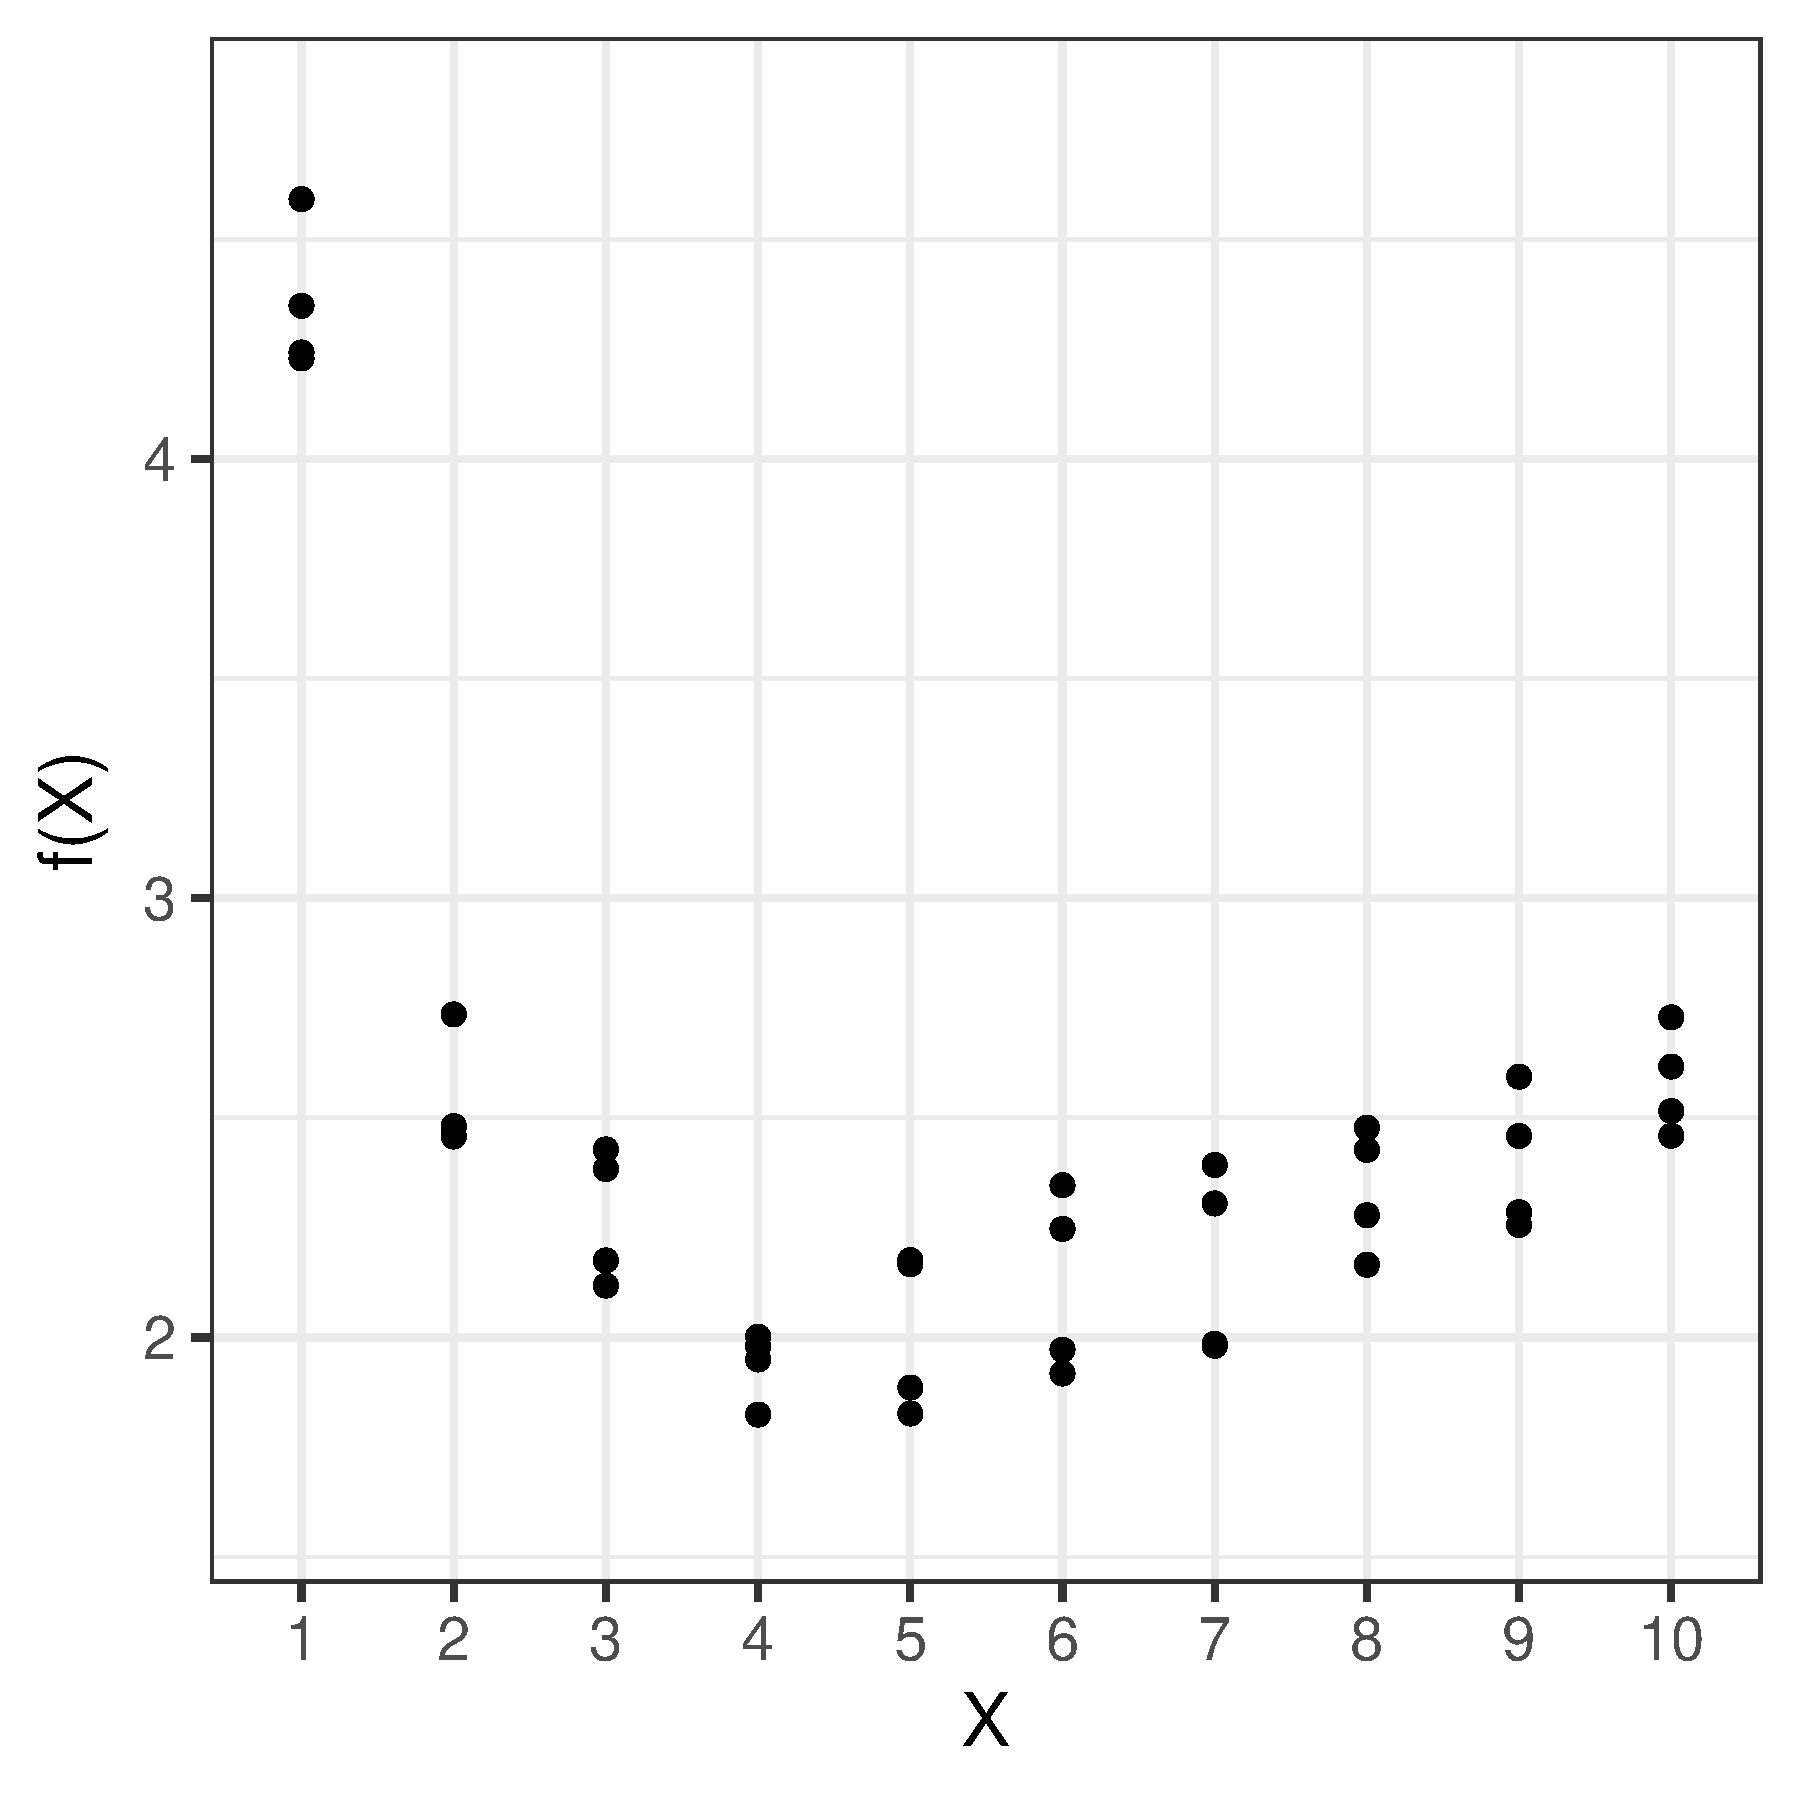
\includegraphics[width=\columnwidth]{../../../img/intro-linear-regression-experimental-data-nomodel.pdf}
\end{center}
}

\only<2>{
\begin{center}
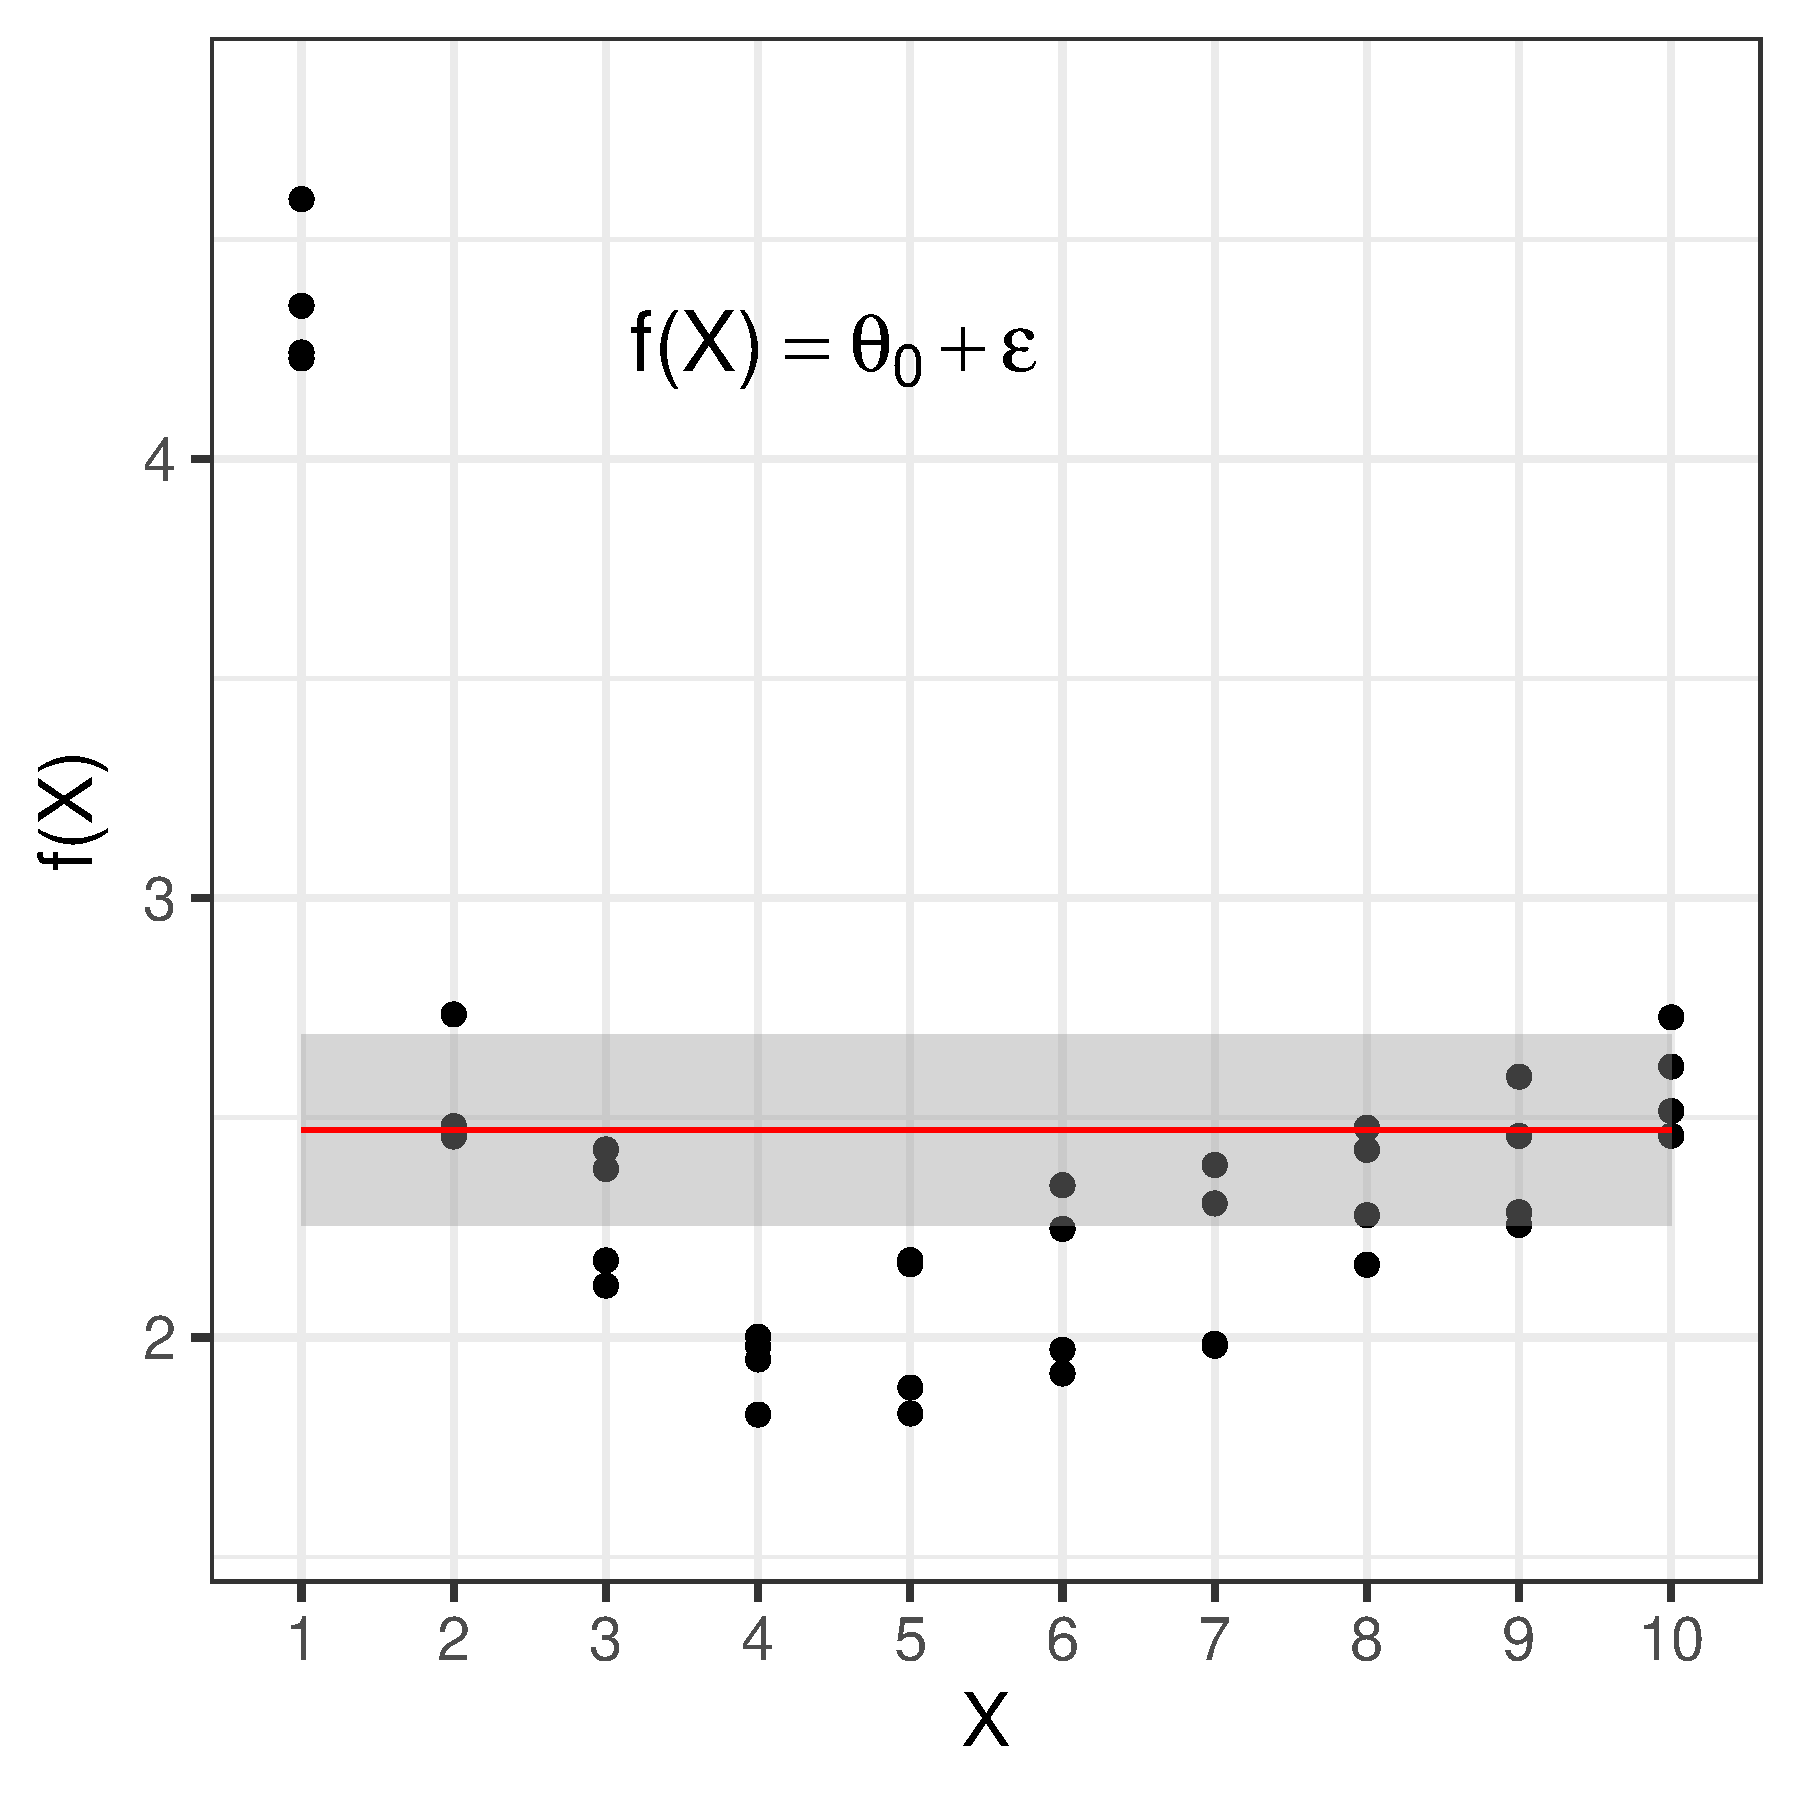
\includegraphics[width=\columnwidth]{../../../img/intro-linear-regression-experimental-data-const-model.pdf}
\end{center}
}

\only<3>{
\begin{center}
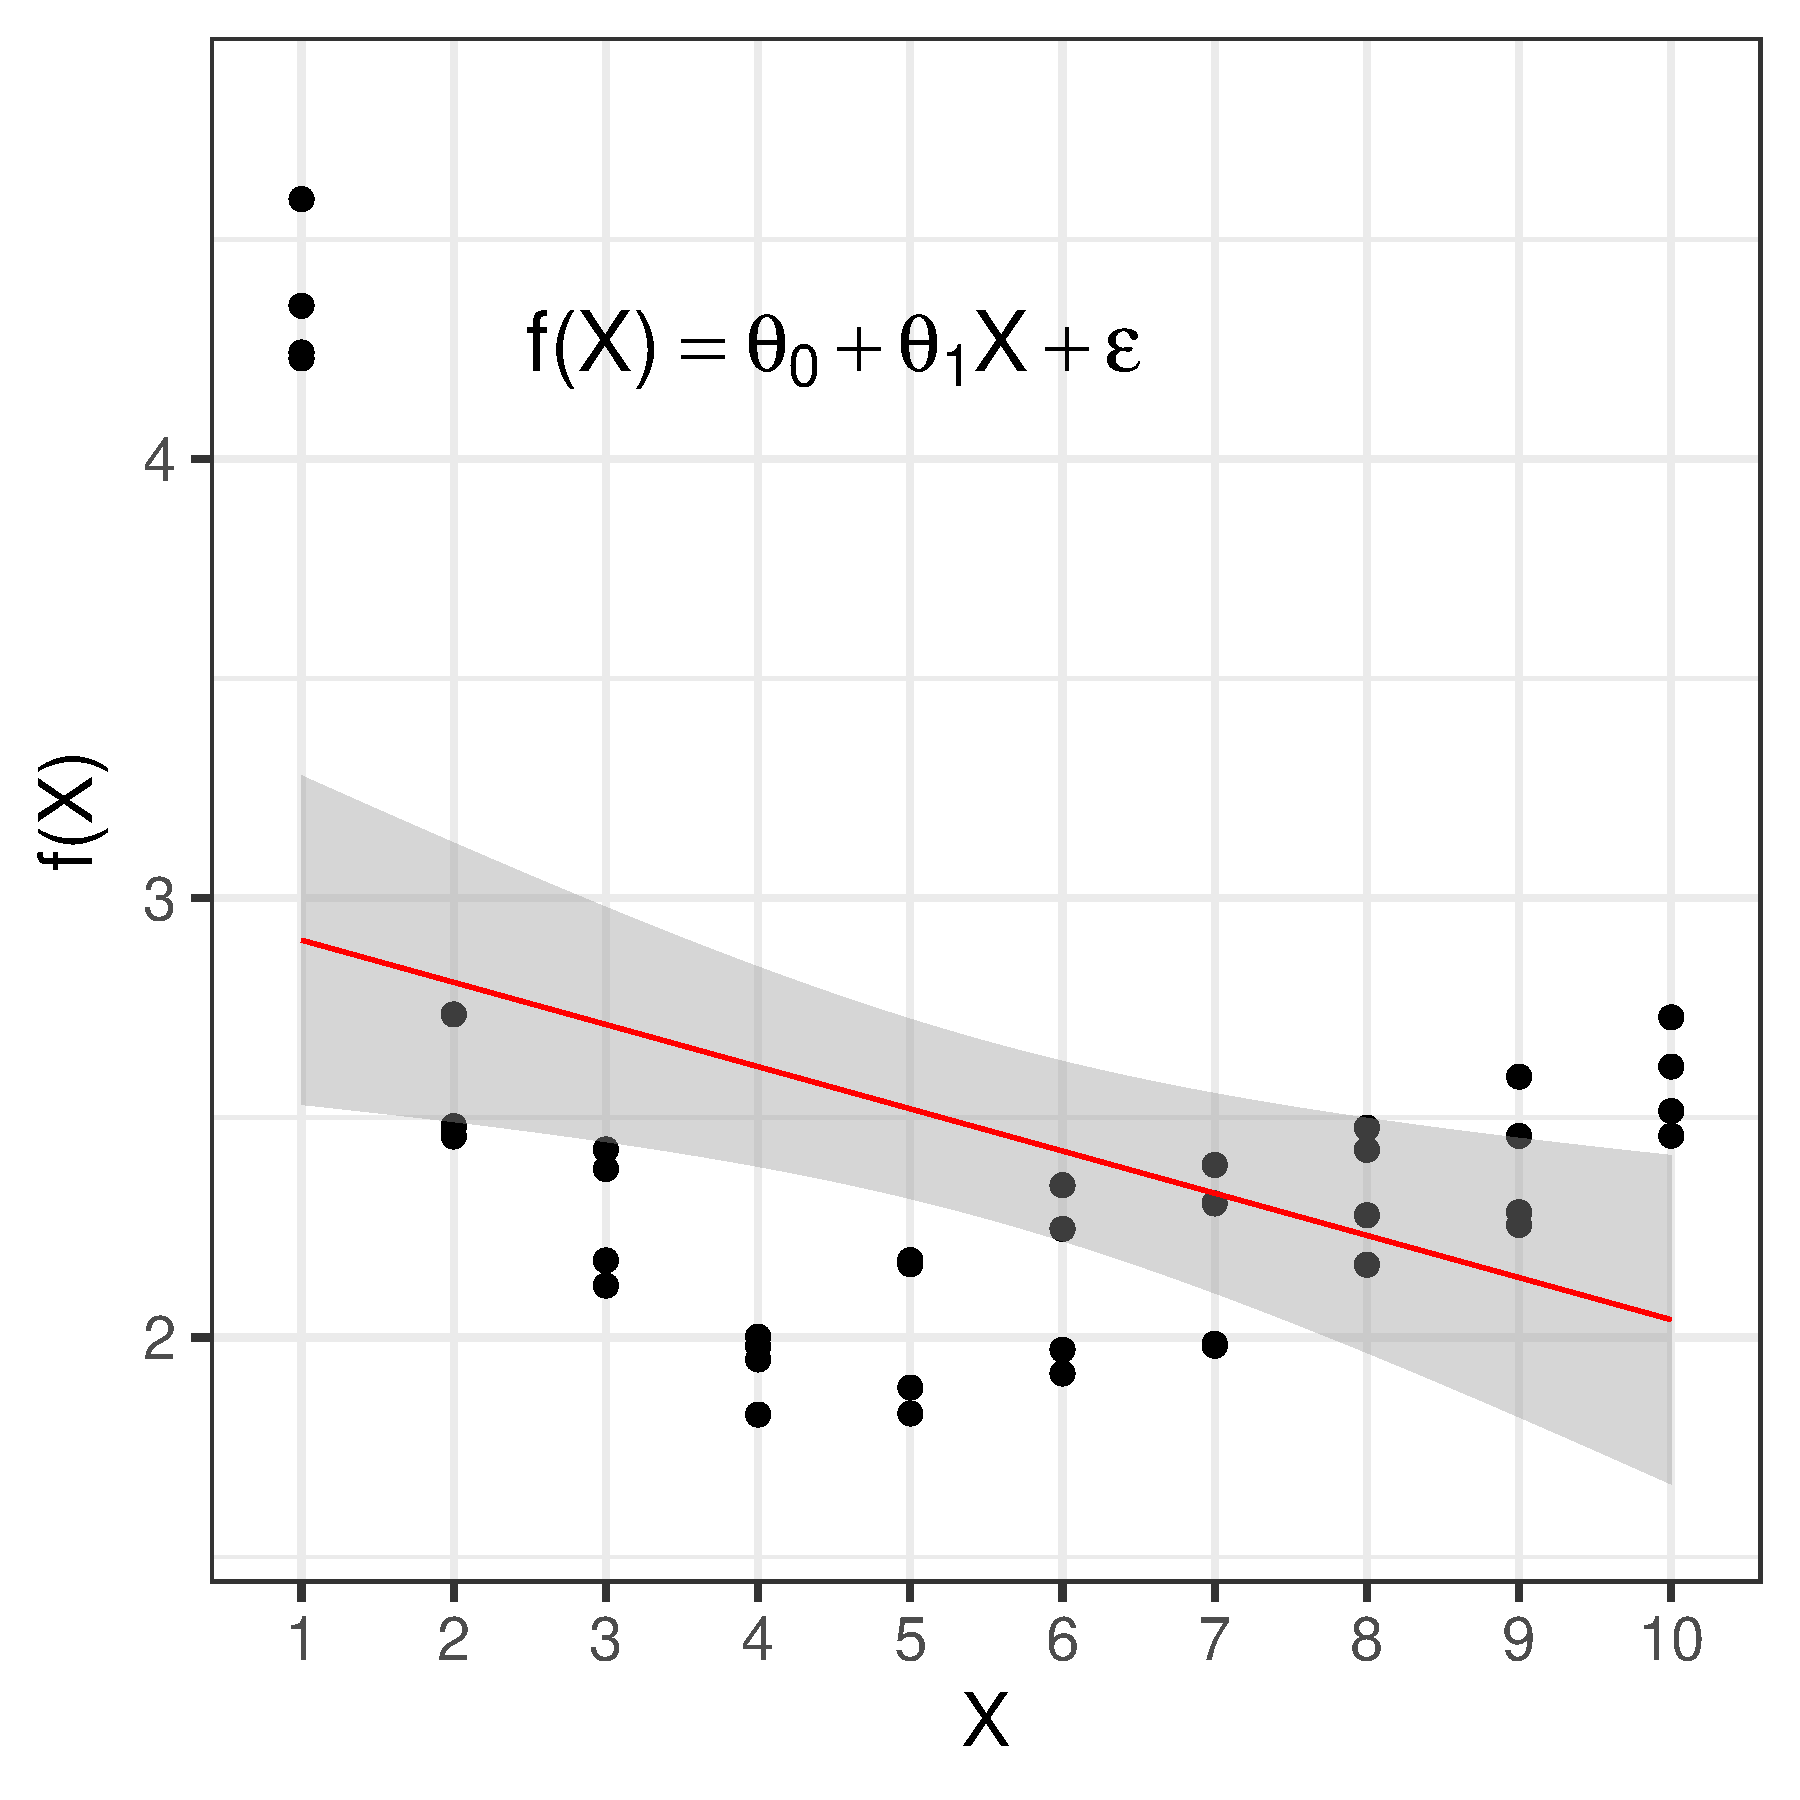
\includegraphics[width=\columnwidth]{../../../img/intro-linear-regression-experimental-data-lin-model.pdf}
\end{center}
}

\only<4>{
\begin{center}
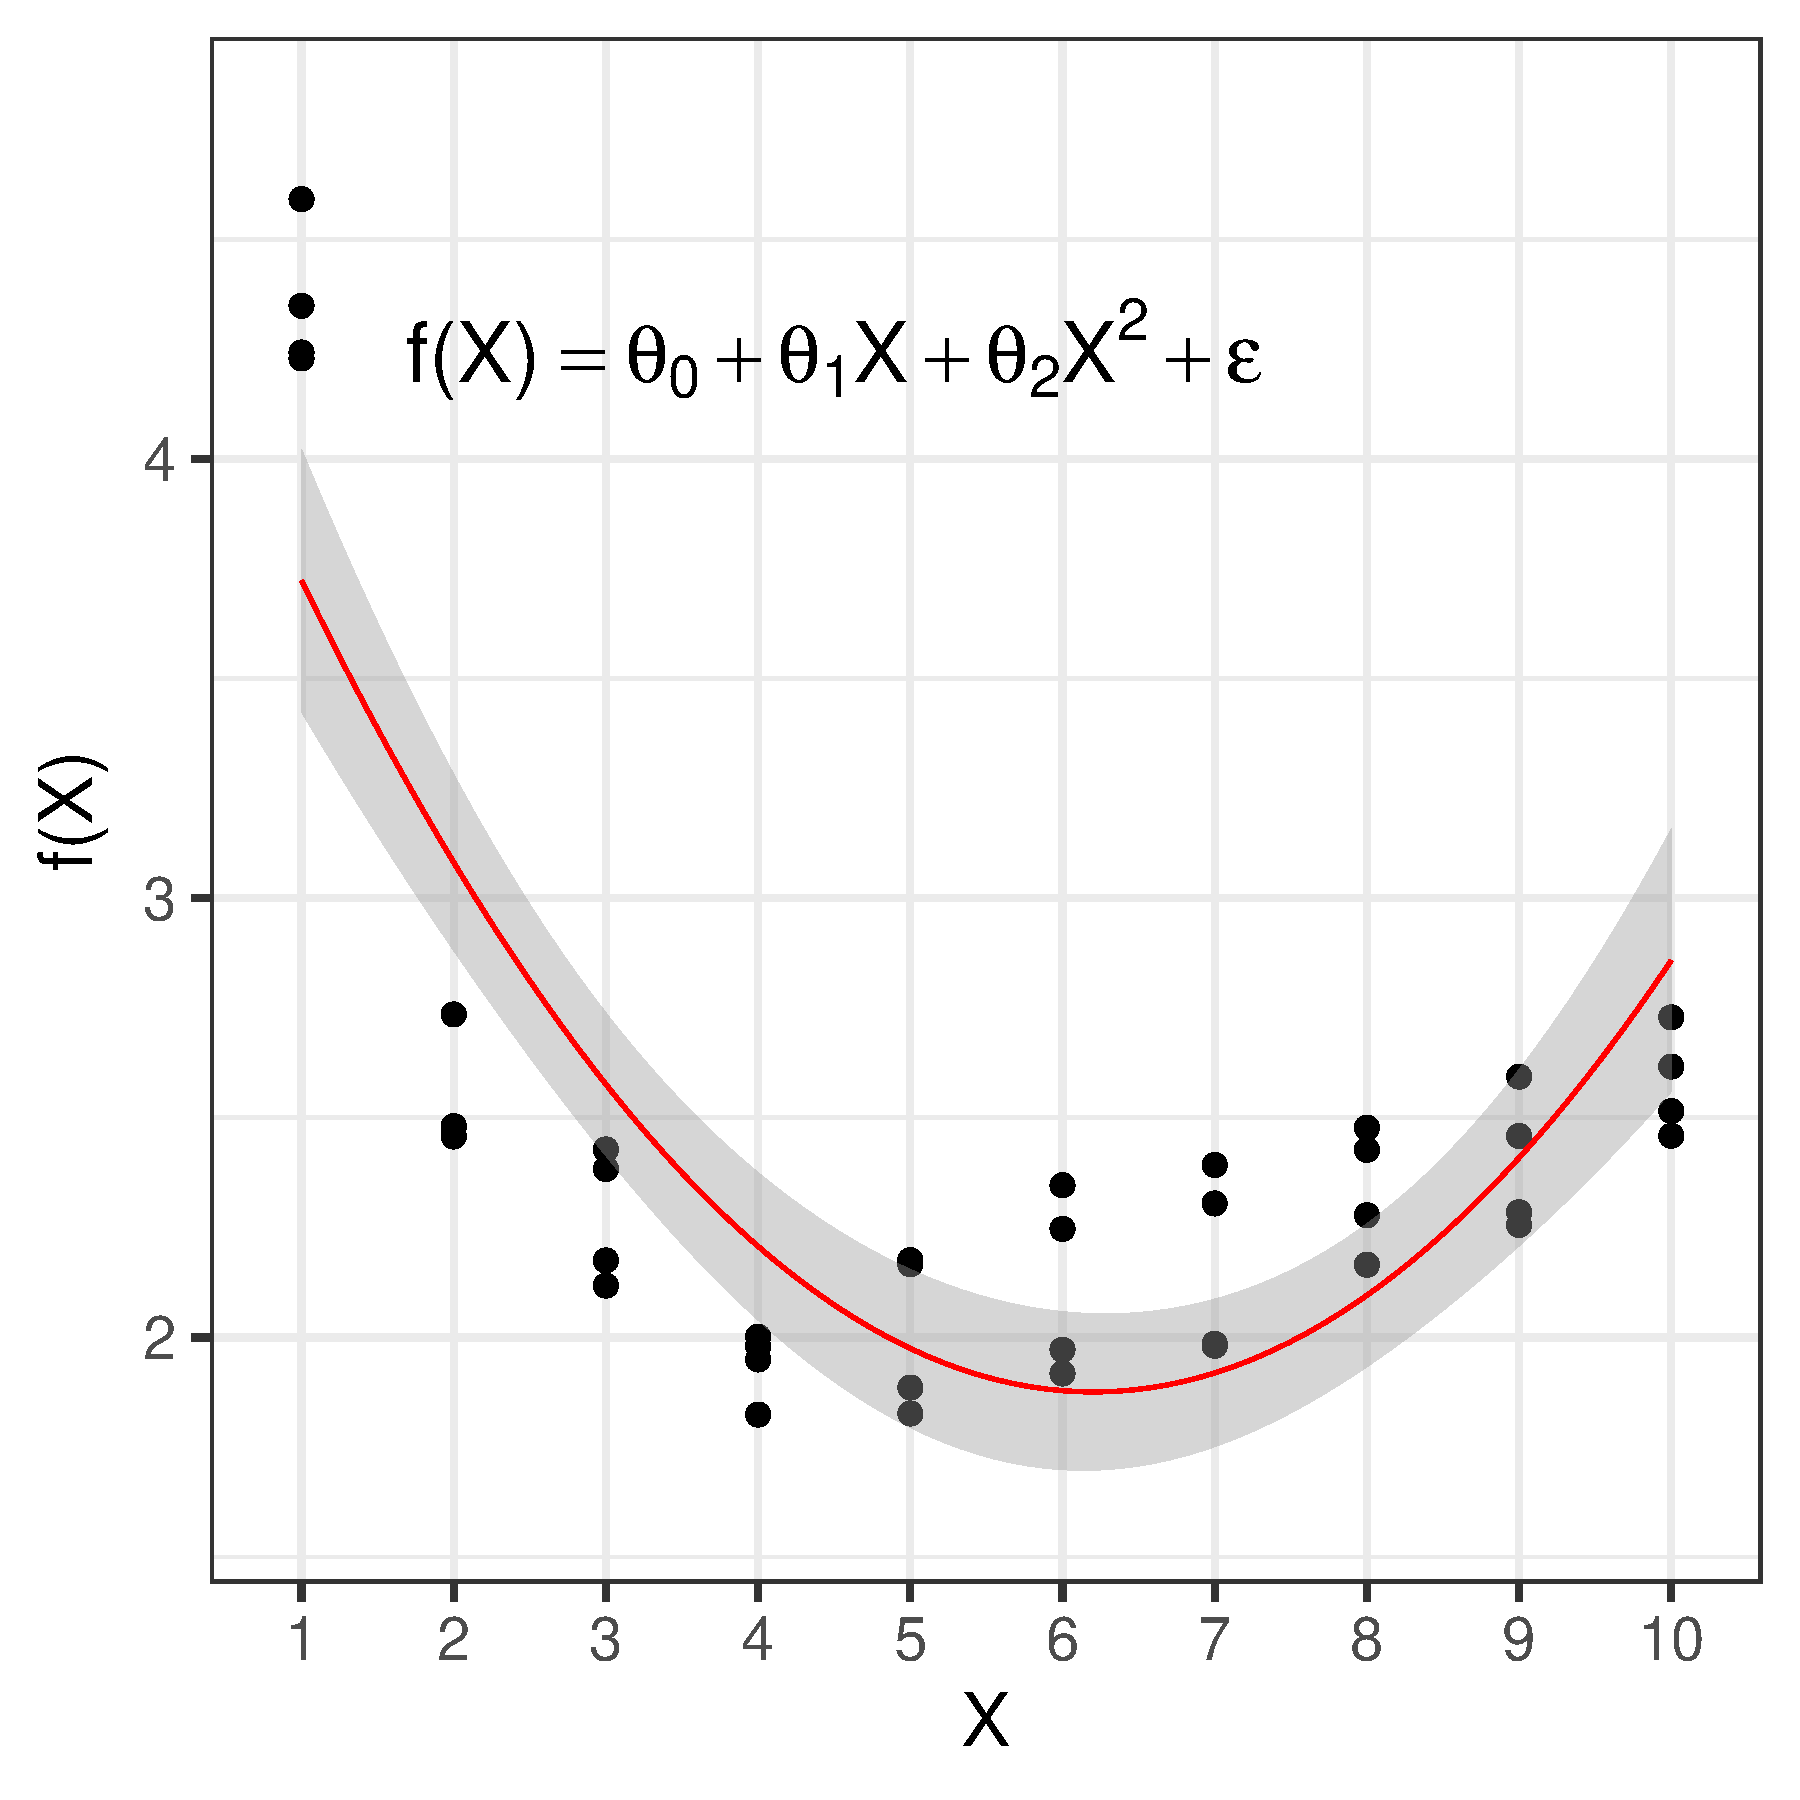
\includegraphics[width=\columnwidth]{../../../img/intro-linear-regression-experimental-data-quad-model.pdf}
\end{center}
}

\only<5->{
\begin{center}
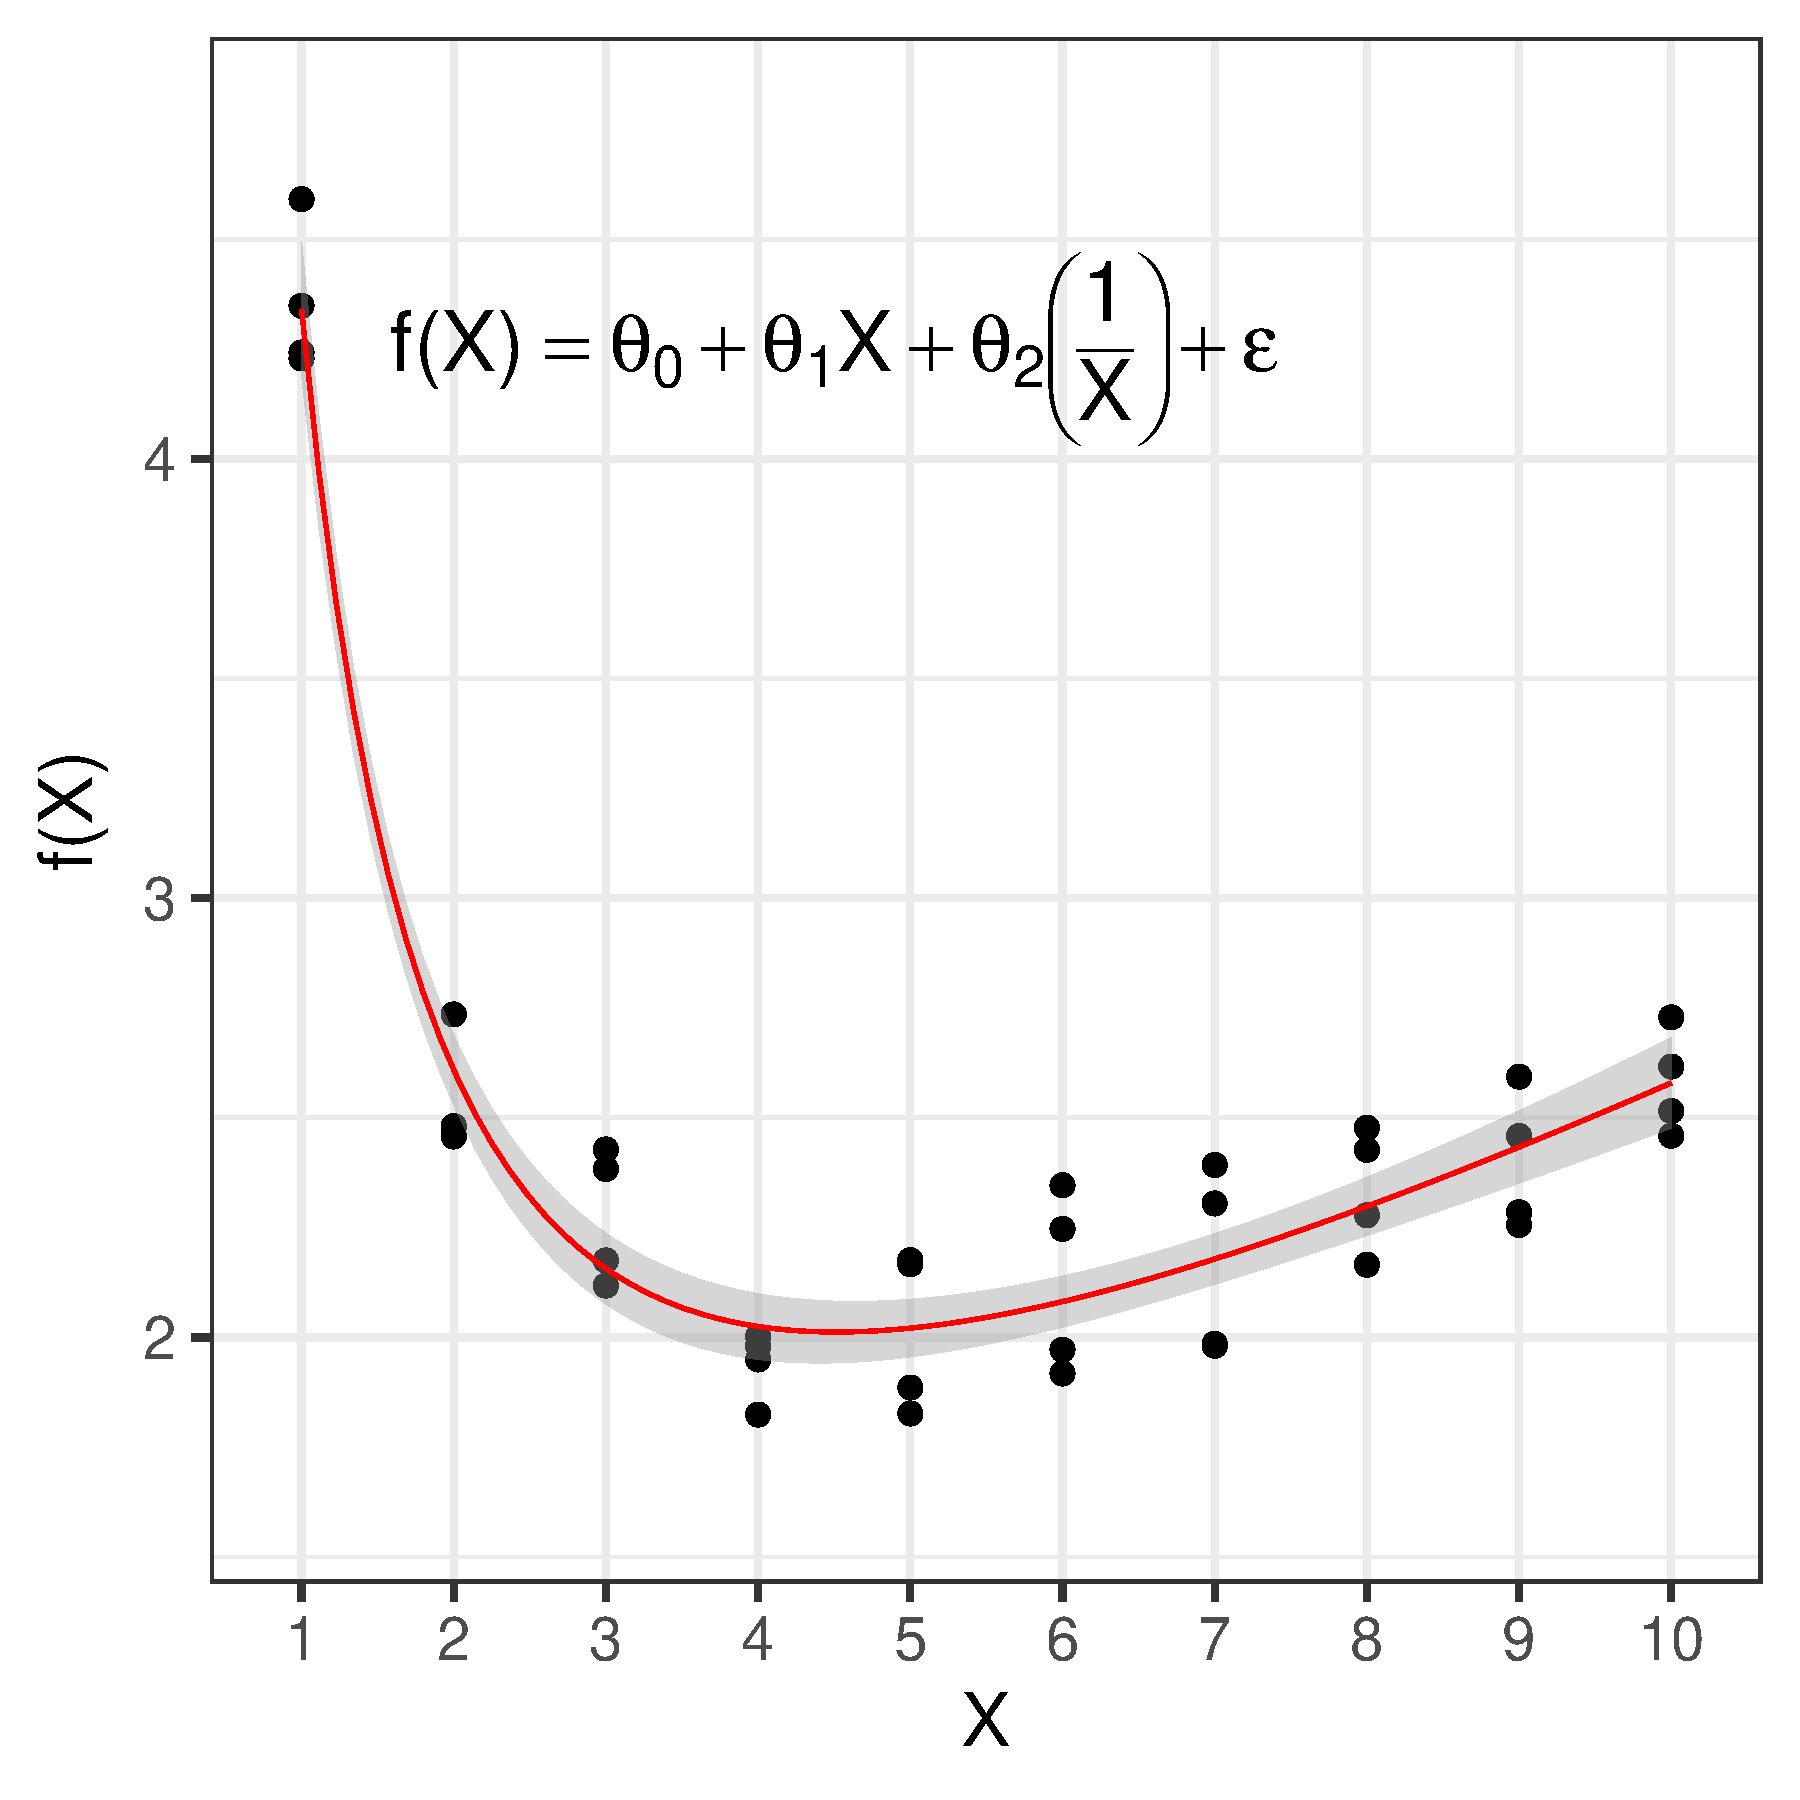
\includegraphics[width=\columnwidth]{../../../img/intro-linear-regression-experimental-data-full-model.pdf}
\end{center}
}
\end{column}
\end{columns}
\end{frame}

\maketitle
\end{document}
